\documentclass[11pt]{article}
\usepackage{final_project}

\usepackage{silence}
\WarningFilter{hyphenat}{*******************************}

\usepackage{todonotes}
\usepackage{microtype}
\usepackage[htt]{hyphenat}
\usepackage{longtable}
\usepackage{pgffor}

\usepackage[utf8]{inputenc} 
% \doublespacing

% \usepackage[nomarkers]{endfloat}

\newcommand{\cp}{\texttt{CartPole}}
\newcommand{\ab}{\texttt{Acrobot}}
\newcommand{\mc}{\texttt{MountainCar}}

\title{State-Space Reduction in Deep Q-Networks}
\author{Michael Ge\thanks{\url{michaelge@college.harvard.edu}} 
        \and 
        Richard Ouyang\thanks{\url{rouyang@college.harvard.edu}}}
\date{\small{\url{https://github.com/hahakumquat/stat234-project}}\\
      April 24, 2018}

\begin{document}

\maketitle

\begin{abstract}
Deep convolutional neural networks have become a popular approach to estimating Q-value functions in reinforcement learning problems. These deep Q-networks take in entire images as network inputs, often resulting in large state spaces and long learning times. In this paper, we explore the use of principal component analysis to reduce the state space of network inputs for small network sizes. After testing multiple network configurations, we determine that a reduction in uninformative state features through PCA helps improve the performance of deep reinforcement learning for small neural network architectures.
\end{abstract}

\newpage
\tableofcontents

\twocolumn
\newpage

\section{Introduction}

Current methods of Q-learning with deep neural networks are inhibited by the large state space inherent in processing images. The state-of-the-art methods used in recent papers \cite{mnih2013playing, mnih2015human, van2016deep} require often infeasible amounts of computational power, time, and data. Although convolutional neural networks theoretically reduce the learning time by restricting the size of the network and accounting for structural information in the data, it is still difficult to learn a good policy in a time- and data-efficient manner. We experiment with reducing the state space dimensionality required by deep Q-networks (DQNs) by applying principal component analysis (PCA) to improve learned policies and training times on a variety of O\-pen\-AI games. Although state-space reduction has previously been studied in reinforcement learning \cite{kishima2013reduction}, use of PCA in reducing state spaces, particularly for neural networks, has not previously been considered. 

In addition, we provide an extensible and easy-to-use software framework to test various types of agents and Q-networks, even for games not tested in this paper (such as Atari games).

\section{Background}

\subsection{MDP Overview}

We will briefly describe the general Markov Decision Process (MDP)
framework. Define an MDP to be a tuple consisting of the following elements:

\begin{itemize}
    \item $\mathcal{S}$, the set of states. In our usage, each state $s \in \mathcal{S}$ is a transformation of the game screens, which are matrices of pixel values.
      
    \item $\mathcal{A}$, the set of actions. The available actions $a \in \mathcal{A}$
    depend on the setting of the game. In the problems of interest, we
    consider games with discrete, relatively simple action spaces.
      
    \item $r: \mathcal{S} \times \mathcal{A} \to \mathbb{R}$, the reward
    function. A reward $r_t(s_t, a_t)$ is given to the agent after an
    action $a_t$ is taken at state $s_t$. The reward is often a complex
    function. If we knew the reward function, we would easily know which
    action to take at any state $s_t$ and timestep $t$.
      
    \item $p: \mathcal{S} \times \mathcal{A} \times \mathcal{S} \to
    \mathbb{R}$, the transition probabilities. After taking action $a$, the agent moves from state $s_t$ to state $s_{t+1}$ with probability $p(s_{t+1} |s_t,
    a_t)$. In our games, transitions are deterministic, so probabilities
    are either $0$ or $1$.
      
    \item $\gamma \in [0, 1]$, the discount factor. $\gamma$ discounts
    future rewards at a constant, compounded rate.
    
    In reinforcement learning, we seek to learn a policy
    $\pi: \mathcal{S} \to \mathcal{A}$ that maximizes the expected
    discounted sum of future rewards at a given state:
    $$R_t = \mathbb{E}\left[\sum_{i=t}^\infty \gamma^{i-t} r_{i}|s_{t-1}\right]$$
    
    We define the Q-function under a policy $\pi$ as the expected
    discounted sum of future rewards given a state and desired action:
    $$Q^\pi(s_t, a_t) = \mathbb{E}\left[R_t | s_{t-1}, a_{t-1} \right]$$
    
    The optimal Q-function has been proven to satisfy the Bellman equation:
    $$Q^\star(s, a) = r(s, a) + \gamma \max_{a' \in \mathcal{A}} Q^\star(s', a')$$
\end{itemize}


\subsection{Deep Q-Networks}

We now briefly discuss the application of deep neural networks to reinforcement learning. The most common use of deep neural networks is to model the Q-function. These deep Q-networks (DQNs) take in a transformed image input $s$, passes it through multiple layers, and returns a vector consisting of the estimated $Q(s, a)$ for all available actions $a \in \mathcal{A}$. 

Current state-of-the-art models \cite{mnih2013playing, mnih2015human} use deep convolutional neural networks (CNNs) as models for the Q-function; these DQNs capitalize on the structure of image data -- for example, correlations between nearby pixels -- to make Q estimates. Unfortunately, DQNs typically require a large number of parameters, thus consuming large amounts of computational resources, in terms of both time and space. In our application, due to computational constraints, we restrict our network architectures to contain about 7000 parameters and briefly explore larger parameter spaces toward the end of the paper. More information about the structure of CNNs is available in Figure \ref{fig:cnn}.

Double DQNs (DDQNs) \cite{van2016deep} are very similar to regular DQNs. However, instead of using the same network to obtain the target value for minibatch updates as in a regular DQN, the DDQN randomly selects one of two networks to update and uses the other network to obtain the target value.

\begin{figure*}
    \centering
    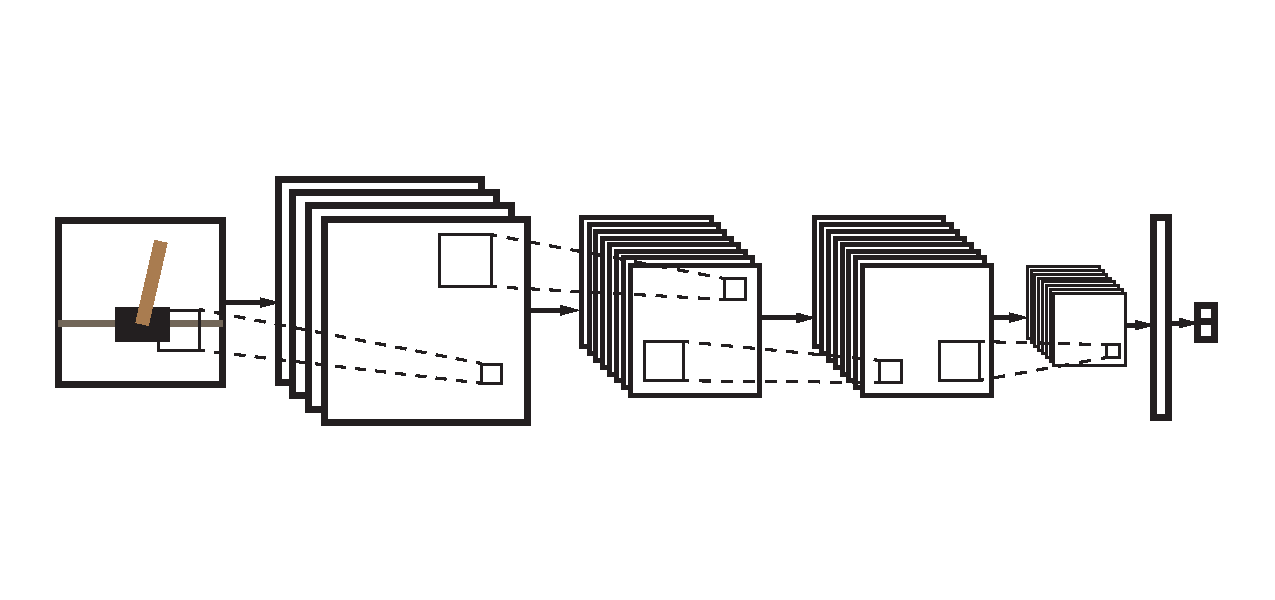
\includegraphics[trim={0 1cm 0 1cm}, clip, width=0.95\textwidth]{cnn.pdf}
    \caption{A visualization of the network structure of a convolutional neural network. The input is the image, which is convolved through several layers, each of which contains several filters. The result is then shrunk through a max pooling layer and passed through a fully connected linear layer before being output as Q-values for each action in the action space.}
    \label{fig:cnn}
\end{figure*}

\subsection{Principal Component Analysis}

Principal component analysis (PCA) is a dimensionality reduction technique that orthogonally projects the original features into a smaller set of features. PCA chooses the axes with the most variance to construct these principal components. Each of the resulting principal components is uncorrelated with and orthogonal to all the other components. In interpreting images, PCA keeps transformations of the most variable pixels, eliminating the information contained in pixels with very little variance.


We briefly describe how PCA works. Consider a setting where we have $n$ state feature vectors $x \in \mathbb{R}^m$. We construct a feature covariance matrix $\mathbf{S}$ as the following:

$$\sum_{i=1}^n x_i x_i^\top = \mathbf{X}^\top \mathbf{X} = \mathbf{S}$$

We then consider the $d$ largest eigenvalues of $\mathbf{S}$. It has been shown that the corresponding eigenvectors of these eigenvalues encompass the maximum amount of variance in the dataset in the subspace $\mathbb{R}^d$. We then construct a $d \times m$ projection matrix $\mathbf{U}$:

$$\mathbf{U} = (\mathbf{u}_1, \ldots, \mathbf{u}_d)^\top$$

For each $\mathbf{x}$, we can then compute the transformed feature vector $\mathbf{z} = \mathbf{U}\mathbf{x}$. These can also be interpreted as the reconstruction coefficients.

To reconstruct a simplified version of the original feature vector, we compute:

$$\hat{\mathbf{x}} = \mathbf{U}^\top \mathbf{z}$$

In our usage, we transform our input images into a feature vector of pixels before performing PCA.


\subsection{OpenAI Gym}

OpenAI Gym \cite{brockman2016openai} offers a set of many standard games on which to test reinforcement learning algorithms. We tested our algorithms, which learn on pixel images, on the following games. See Figure \ref{fig:game_images} for sample images of each game.

\begin{description}
    \item[\href{https://gym.openai.com/envs/CartPole-v0/}{CartPole-v0}] \cp~is the classic reinforcement learning environment. At every time step, the agent receives a reward of $1$ and chooses to push the cart either right or left. The game ends when the pole falls to an angle greater than 15 degrees from vertical or when the cart moves off the screen. 
    \item[\href{https://gym.openai.com/envs/Acrobot-v1/}{Acrobot-v1}] \ab~is a reinforcement learning game consisting of a double pendulum. The agent can only apply force to the connecting joint (left, right, or no movement) and must swing the pendulum so that the tip of the pendulum reaches a certain height. The agent receives a reward of $-1$ for every time step the goal is not reached.
    \item[\href{https://gym.openai.com/envs/MountainCar-v0/}{MountainCar-v0}] \mc~is a reinforcement learning game in which the agent tries to drive a car up a hill. The car is not strong enough to climb the hill itself and thus must learn to use gravity to achieve the necessary speed. At every time step, the three movements available are accelerating to the right, accelerating to the left, and doing nothing. The agent receives a reward of $-1$ for every time step the goal is not reached. 
\end{description}

\begin{figure*}[!ht]
\centering
\foreach \imagetype in {original, processed}
{
    \subfloat[Sample \imagetype~image of the \cp~game screen. ]{%
        \includegraphics[width=0.30\textwidth]{game_images/CartPole_\imagetype.pdf}
        \label{subfig:CartPole_\imagetype}
    }
    \hfill
    \subfloat[Sample \imagetype~image of the \ab~game screen. ]{%
        \includegraphics[width=0.30\textwidth]{game_images/Acrobot_\imagetype.pdf}
        \label{subfig:Acrobot_\imagetype}
    }
    \hfill
    \subfloat[Sample \imagetype~image of the \mc~game screen. ]{%
        \includegraphics[width=0.30\textwidth]{game_images/MountainCar_\imagetype.pdf}
        \label{subfig:MountainCar_\imagetype}
    }
}
\caption{Original and processed images from the three games discussed in this paper. The processed images were created by grayscaling the original images and resizing from $600 \times 400$ pixels to $80 \times 80$ pixels. The resulting feature space is then $\mathbb{R}^{6400}$.}
\label{fig:game_images}
\end{figure*}

\subsection{PyTorch}

PyTorch \cite{paszke2017pytorch} is a Python framework for constructing neural network architectures. Although PyTorch is still in its early stages of development, it has several advantages compared to other neural network libraries such as TensorFlow and Keras. Namely, improvements include a clean extension of the common Python package \texttt{NumPy}, deep integration with Python, and efficient memory usage. 

\section{Methods}

\subsection{Initial Setup}

We replicated the original deep Q-network papers \cite{mnih2013playing, mnih2015human} in Python, using PyTorch \cite{paszke2017pytorch} for the neural network architecture and OpenAI Gym \cite{brockman2016openai} to test and compare our algorithms on different games. 

There are quite a few steps to get started to replicate our procedure, including changing some of the source code in OpenAI Gym. For the sake of brevity, these instructions are included in Appendix \ref{app:getting_started}. To run our experiments, we used a limited partition of an Odyssey research computing cluster to run a portion of our computationally intensive jobs.

\subsection{Image Preprocessing}

In this project, our goal was to learn the optimal policy for the games without using parametric data -- for example, the pole angle in \cp. Instead, we focused more on image processing rather than using the state information given by the Gym environment.

At each time step, we obtained the RGB (color) mapping of the game screen, resized the image to $80 \times 80$ pixels (rectangular images were squashed into a square), and converted the image to grayscale. We then took the difference between the current timestep's image and the last timestep's image as the state to input into our DQN. 

\subsection{Model Structures}
\label{subsec:model_structure}

In our experiments, we used four different types of models, each of which includes the original and double network variants: 

\begin{description}
    \item[(D)DQCNN] The original model \cite{mnih2013playing, mnih2015human} and variants \cite{van2016deep}. These models convolve images using no extra state-space reduction techniques like PCA. This model is also referred to as (D)DQN-GS, since this is the original grayscale model. We use these two terms interchangeably.
    
    \item[(D)DQN-PCA] These models use a database of 1000 states, generated from a random policy, as training data for PCA and project the pixel features of new states onto the subspace that captures at least 99\% of the variance. The results is a one-dimensional vector with varying lengths based on the game (100 to 500 features). This vector is passed into a feed-forward (not convolutional) deep neural network with varying numbers of layers and nodes to predict the Q-value.
    
    \item[(D)DQCNN-PCA] These models also perform PCA; however, the (D)DQCNN-PCA models then invert the PCA transformation, converting each transformed image back to its original space. The result is a simplified $80 \times 80$ image, which is then input into a model with the same network structure as the original (D)DQN.
    
    \item[(D)DQCNN-PCA-Mini] Out of curiosity, we included one additional model type, which takes the one-dimensional vector obtained from the PCA transformation and reshapes it into a square (zero padding if necessary). We then convolved the resulting ``image'' through a smaller neural network to predict the Q-value for each state. Although PCA strips correlation between nearby pixels, we were interested in investigating whether the reduced dimensionality preserved some structure between nearby values.
\end{description}

For the (D)DQCNN and (D)DQCNN-PCA models, we kept our network structure similar but reduced in parameter size to \cite{mnih2013playing} and \cite{mnih2015human} by using three hidden layers in each network. These DQNs take in an $80 \times 80$ grayscale image. Each hidden layer in the network convolves the previous layer's output into multiple filters, followed by a batch normalization and a leaky ReLU with $\alpha = 0.001$ to prevent dead nodes. The first layer convolves $8$ $8 \times 8$ filters with stride $4$; the second layer convolves $16$ $4 \times 4$ filters with stride $2$; the final hidden layer convolves $16$ $4 \times 4$ filters, this time with stride $1$. A max pooling with kernel size $2$ is then applied to reduce the dimensionality of the output. The final layer is fully connected and maps linearly to the number of actions available. For instance, since \cp~contains two actions at any time, the output of the neural network contains two nodes. This structure saves time when forwarding through the network, since a single forward pass for a given state $s$ gives $\hat{Q}_\text{network}(s, a)$ for all $a \in \mathcal{A}$. The images can be found in \ref{fig:pca_images}.

To ensure that the models are relatively comparable, we kept the number of parameters for each model as close as possible at around 7,000 parameters. For the (D)DQN-PCA model, we tested a variety of network architectures, varying the number of layers as well as the number of nodes in each layer. 

For the (D)DQCNN-PCA-Mini model, we kept the rough network structure the same as our original models. However, to account for the smaller image size, we reduced the kernel size to 4 and the stride to 1 for all layers.

\begin{figure*}[!ht]
\centering
\foreach \pca in {DQCNN-PCA, DQCNN-PCA-Mini}
{
    \subfloat[Sample PCA-transformed image of the \cp~game screen for the \pca~model. ]{%
        \includegraphics[width=0.30\textwidth]{game_images/CartPole_\pca.pdf}
        \label{subfig:cartpole_\pca_image}
    }
    \hfill
    \subfloat[Sample PCA-transformed image of the \ab~game screen for the \pca~model. ]{%
        \includegraphics[width=0.30\textwidth]{game_images/Acrobot_\pca.pdf}
        \label{subfig:acrobot_\pca_image}
    }
    \hfill
    \subfloat[Sample PCA-transformed image of the \mc~game screen for the \pca~model. ]{%
        \includegraphics[width=0.30\textwidth]{game_images/MountainCar_\pca.pdf}
        \label{subfig:mountaincar_\pca_image}
    }
}
\caption{PCA images from the three games discussed in this paper. The PCA images were created by grayscaling the original images, using the features that capture 99\% of the variance, and either inverting the transformation or not. The resulting feature space depends on the PCA reduction amount. Note that the most important pixels (near the game object in the first row, and near the top in the second row) are much more variable in color than the less important pixels, which tend to be a relatively uniform gray.}
\label{fig:pca_images}
\end{figure*}

\subsection{Hyperparameters}

We tested many configurations of hyperparameters, varying the following: 

\begin{description}
    \item[Model] One of the Q-function models mentioned in Section \ref{subsec:model_structure}.
    
    \item[Frame skip] The number of time steps for which the same action is repeated. To speed up learning, we used this method described in \cite{mnih2013playing, mnih2015human}. When an action is selected, that action is repeated for the next $k$ frames, since selecting an action and training takes much more time than rendering an additional step of the game. We chose $k = 3$ since $k = 4$, which was suggested in \cite{mnih2013playing, mnih2015human}, empirically performed worse in \cp. 
    
    \item[Update frequency] The number of distinct action selections between each minibatch update. This value is typically set to $4$. This technique speeds up the training even further, since rendering the environment is far less costly than forwarding through the network. This has been used in other papers \cite{mnih2013playing, mnih2015human, van2016deep}.
    
    \item[Number of training steps] The length of time the model should be trained, expressed in terms of the number of minibatch training steps. While state-of-the-art research uses up to 10 million frames, our resources restrict us to values between 10 thousand and 100 thousand.
    
    \item[Replay memory size] The maximum number of transitions -- each of which is a $(s, a, r, s')$ tuple -- stored in the replay memory. The replay memory is used to reduce correlation between transitions used in each minibatch update \cite{mnih2013playing, mnih2015human}.
    
    \item[Target update] If the model uses a target network \cite{mnih2015human}, this represents the number of trains between each target network update. Each update involves setting the target network parameters to the main network parameters.
    
    \item[Learning rate] The (initial) learning rate used by the optimizer. A higher learning rate results in a model that learns faster but may diverge.
    
    \item[Learning rate annealing] Whether the learning rate is annealed to a smaller value. Learning rate annealing helps decrease the likelihood of policy divergence. The learning rate anneals according to the equation $$\alpha_t = \alpha_\text{initial} \max\left(\exp\left(-\frac{t}{\lambda_\alpha}\right), \frac{0.0005}{\alpha_\text{initial}}\right),$$ where $t$ is the number of minibatch training updates that have already occurred, and $\lambda$ is the decay rate, so that the learning rate anneals exponentially from its initial value to a final value of $0.0005$.
    
    \item[Batch size] The minibatch size, or the number of transitions used in each training update. The two values tested were $32$ and $128$.
    
    \item[Loss function] The loss function used in the model. The Huber loss (defined as the $\ell_2$ norm for losses greater than 1 and the $\ell_1$ norm otherwise) and the mean squared error (MSE) loss were the two loss functions considered.
    
    \item[Regularization] The weight decay in the optimizer. This value typically ranges from $0$ to $1$ and is used to prevent overfitting in our networks.
    
    \item[Agent action selection] We used an $\epsilon$-greedy agent, annealing $\epsilon$ from $\epsilon_\text{initial} = 1$ to $\epsilon_\text{final} = 0.1$ according to the equation $$\epsilon_t = \epsilon_\text{final} + (\epsilon_\text{initial} - \epsilon_\text{final}) \exp\left(-\frac{t}{\lambda_\epsilon}\right),$$ where $t$ is the number of times the agent has already selected an action, and $\lambda$ is the decay rate. 
    
    \item[Network Architecture] Toward the end of our experimentation, we had the time to test different network configurations for the (D)DQN-PCA model. Unfortunately, due to the computational demands of performing over images, it was intractable to test larger node structures.
\end{description}

\subsection{Implementation Details}

The code is structured such that the user can pass a model, agent, game, and a large selection of hyperparameters into \texttt{main.py}. During the script execution, statistics are logged for later analysis. 

Within our \path{utils/} folder, we implemented several scripts to aid in the data analysis process, some of which we will briefly discuss here. 

\begin{itemize}
    \item \texttt{Logger.py} is a general logging utility for storing statistics in files. 
    \item \texttt{PCA.py} contains a PCA class whose objects can train on inputs of states, return the transformed features, and invert already-transformed features back into the original image space. 
    \item \texttt{ReplayMemory.py} contains a class whose objects store and quickly sample transitions for minibatch updates. 
    \item \path{get_notes_and_stats.py} parses our raw data into an easy-to-read format, providing summary statistics, hyperparameters, and metadata about each job. 
    \item \path{plot_data.py} plots raw data as well as running means over episodes and training updates. 
    \item \path{save_states.py} runs a random policy for each game, saving a large set of states on which PCA can later be performed. 
\end{itemize}
 
Our \path{automate_run} folder contains the following bash scripts for running jobs on the computing cluster:

\begin{itemize}
    \item \path{gen_slurms.sh} and \path{search_nets.sh} iterate over a given hyperparameter space and submit batch jobs for each hyperparameter combination in parallel.
    \item \path{view_plots.sh} is a utility that allows the user to view the rewards of each game, providing a preliminary categorization of model performance. 
\end{itemize}

Although we did have access to a computing cluster, the access was limited and we did not have access to GPUs, which significantly speed up learning for neural networks. We also had limited time to run our experiments, preventing us from running the 10 million frames per game prescribed in the literature \cite{mnih2013playing, mnih2015human}. This was the motivation for our efforts to improve learning by reducing the state space.

\section{Results}

The full set of raw data, metadata, and plots are available at this \href{https://github.com/hahakumquat/stat234-project/tree/master/data}{link} (warning: approximately 600 MB). For all our experiments, our primary measure of policy performance was the mean reward over the second half of the episodes, with a rolling mean over the previous 5\% of the total number of episodes providing a similar but smoother representation of model performance.

All summary statistics are taken over the second half of the experiment, after the algorithm has had time to learn the game and converge. This prevents the learning process from affecting measurements of the final learned policy.

Note that these plots are graphed across all of the episodes completed within a constant number of training iterations. Therefore, note that the number of episodes varies depending on the durations of each game. That is, for longer game durations, we have fewer episodes. For the sake of comparison within games, the $y$-axes for the reward graphs are standardized, even if episode rewards are outside the axis limits. In particular, the $y$-axis is clipped to be between 0 and 200 for \cp, $-2000$ and 0 for \ab, and $-5000$ and 0 for \mc. We do this because unclipped axes often create difficulties in detecting patterns in regions with low reward variance. 

One notable yet intentional quirk of our data collection scheme is the fact that each of our trials contains a different number of episodes, even when considering models within the same game. This difference occurs because we seek to keep training time constant between models. For instance, if we were to train models for a constant number of episodes, a poor \mc~model that averages episode durations around 5000 (and thus per-episode rewards around -5000) would be able to use approximately ten times more training time (measured in clock time) than a better \mc~model that averages episode durations around 500 (and thus per-episode rewards around -500). On the other hand, by training models for a constant number of training steps, we ensure that training time as well as the number of minibatch updates is relatively constant between all models. This strategy is consistent with the deep Q-learning literature \cite{mnih2013playing, mnih2015human, van2016deep}, which typically keeps the number of frames played constant.

\subsection{Random Policy}

As a baseline, we ran a random policy on each game, with results in Figures \ref{fig:CartPole_random}, \ref{fig:Acrobot_random}, and \ref{fig:MountainCar_random}. The average rewards and durations for the three games are available in Table \ref{tab:random_rewards}. With this initial goal in mind, we proceeded to test different model architectures and hyperparameter settings to achieve good empirical results over all three games.

\foreach \game in {CartPole, Acrobot, MountainCar}
{
    \begin{figure*}[!ht]
        \centering
        \subfloat[Rewards by episode, as well as a rolling mean, for a random policy in the \texttt{\game}~game. ]{%
            \includegraphics[width=0.45\textwidth]{\game/\game_NoTraining_Random_rewards.pdf}
            \label{subfig:\game_NoTraining_Random_rewards}
        }
        \hfill
        \subfloat[Durations by episode, as well as a rolling mean, for a random policy in the \texttt{\game}~game.]{%
            \includegraphics[width=0.45\textwidth]{\game/\game_NoTraining_Random_durations.pdf}
            \label{subfig:\game_NoTraining_Random_duraions}
        }
    \caption{Baseline results from the \texttt{\game}~game from OpenAI Gym under a random policy.}
    \label{fig:\game_random}
    \end{figure*}
}

\begin{table*}[!ht]
    \footnotesize
    \centering
    \begin{tabular}{c|cc}
        \toprule
        Game & Average Duration & Average Reward \\ \midrule
        CartPole-v0 & 18.441 & 18.441 \\
        Acrobot-v1 & 599.73 & -598.73 \\
        MountainCar-v0 & 2717.77 & -2717.77 \\
        \bottomrule
    \end{tabular}
    \caption{Average rewards and durations under a random policy for the three games.}
    \label{tab:random_rewards}
\end{table*}

% \subsection{Initial Exploration}

% Although \cite{mnih2013playing, mnih2015human} used a learning rate of $0.00025$, we found that learning was far too slow for our purposes and instead opted for a larger learning rate. We began with a learning rate of $0.1$, but this was far too large: CartPole would learn to durations of around 200 time steps within a few dozen iterations but would quickly diverge. The other two games also did not converge. Significant improvements occurred after reducing to a learning rate of about $0.001$. 

% We used

% \begin{itemize}
%     \item \cp~learning rate 001
% \end{itemize}

\subsection{Hyperparameter Tuning Results}

In our hyperparameter tuning, we decided to keep the frame skip, update frequency, replay memory size, and agent action selection hyperparameters constant for testing, since grid search sizes increase exponentially in the number of parameters, and varying these settings would vastly increase simulation time and space consumption. 

\subsubsection{First Grid Search (10,000 Iterations)}

In order to establish a solid set of hyperparameters to which PCA variants of DQNs could be compared, we began our experiments with an initial grid search over the hyperparameters of interest for 10,000 training steps to eliminate poorly performing hyperparameter settings. Table \ref{tab:grid_search_v1_10k} contains the results of the top fifteen models for each game ordered by performance.

\begin{table*}[!ht]
    \footnotesize
    \centering
    \begin{tabular}{rrlllrllr}
\toprule
   mean &     std &            game &    model & target &      lr & lr\_anneal & loss\_function &  weight\_decay \\
\midrule
-194.65 &   40.72 &  MountainCar-v0 &  DDQN\_GS &    N/A &  0.0010 &     False &         Huber &         0.100 \\
-203.34 &   51.92 &  MountainCar-v0 &  DDQN\_GS &    N/A &  0.0010 &     False &         Huber &         0.001 \\
-275.30 &  143.07 &  MountainCar-v0 &   DQN\_GS &  False &  0.0010 &     False &         Huber &         0.100 \\
-401.52 &  174.12 &  MountainCar-v0 &  DDQN\_GS &    N/A &  0.0010 &     False &         Huber &         0.001 \\
-432.88 &  184.60 &  MountainCar-v0 &  DDQN\_GS &    N/A &  0.0010 &     False &         Huber &         0.100 \\
-447.00 &  188.12 &  MountainCar-v0 &   DQN\_GS &  False &  0.0010 &     False &         Huber &         0.001 \\
-459.67 &  203.96 &  MountainCar-v0 &  DDQN\_GS &    N/A &  0.0010 &      True &         Huber &         0.001 \\
-515.18 &  260.42 &  MountainCar-v0 &  DDQN\_GS &    N/A &  0.0001 &      True &         Huber &         0.100 \\
-741.46 &  475.74 &  MountainCar-v0 &   DQN\_GS &   True &  0.0010 &     False &         Huber &         0.001 \\
-747.50 &  485.40 &  MountainCar-v0 &   DQN\_GS &   True &  0.0010 &     False &           MSE &         0.100 \\
-767.06 &  544.14 &  MountainCar-v0 &   DQN\_GS &   True &  0.0010 &     False &           MSE &         0.100 \\
-779.10 &  593.02 &  MountainCar-v0 &   DQN\_GS &   True &  0.0010 &      True &           MSE &         0.100 \\
-815.88 &  514.64 &  MountainCar-v0 &   DQN\_GS &   True &  0.0010 &     False &         Huber &         0.100 \\
-819.31 &  400.22 &  MountainCar-v0 &  DDQN\_GS &    N/A &  0.0001 &      True &         Huber &         0.100 \\
-830.99 &  585.96 &  MountainCar-v0 &   DQN\_GS &   True &  0.0010 &      True &           MSE &         0.100 \\
  45.09 &   20.87 &     CartPole-v0 &  DDQN\_GS &    N/A &  0.0010 &     False &         Huber &         0.100 \\
  43.74 &   18.85 &     CartPole-v0 &  DDQN\_GS &    N/A &  0.0010 &      True &         Huber &         0.100 \\
  42.95 &   20.65 &     CartPole-v0 &  DDQN\_GS &    N/A &  0.0010 &     False &         Huber &         0.100 \\
  41.33 &   20.06 &     CartPole-v0 &  DDQN\_GS &    N/A &  0.0010 &     False &         Huber &         0.001 \\
  41.02 &   17.93 &     CartPole-v0 &  DDQN\_GS &    N/A &  0.0001 &     False &           MSE &         0.100 \\
  38.56 &   20.58 &     CartPole-v0 &  DDQN\_GS &    N/A &  0.0010 &      True &         Huber &         0.001 \\
  36.85 &   19.40 &     CartPole-v0 &  DDQN\_GS &    N/A &  0.0001 &      True &         Huber &         0.001 \\
  35.95 &   20.28 &     CartPole-v0 &   DQN\_GS &  False &  0.0001 &      True &         Huber &         0.100 \\
  34.19 &   19.59 &     CartPole-v0 &  DDQN\_GS &    N/A &  0.0010 &     False &         Huber &         0.100 \\
  34.05 &   18.31 &     CartPole-v0 &  DDQN\_GS &    N/A &  0.0001 &     False &         Huber &         0.100 \\
  32.99 &   18.97 &     CartPole-v0 &  DDQN\_GS &    N/A &  0.0010 &      True &         Huber &         0.001 \\
  32.15 &   18.75 &     CartPole-v0 &   DQN\_GS &  False &  0.0010 &     False &         Huber &         0.001 \\
  31.80 &   18.42 &     CartPole-v0 &  DDQN\_GS &    N/A &  0.0010 &      True &         Huber &         0.001 \\
  31.65 &   18.50 &     CartPole-v0 &  DDQN\_GS &    N/A &  0.0010 &      True &         Huber &         0.100 \\
  31.13 &   17.34 &     CartPole-v0 &   DQN\_GS &  False &  0.0001 &     False &         Huber &         0.100 \\
-135.35 &   40.45 &      Acrobot-v1 &  DDQN\_GS &    N/A &  0.0010 &     False &         Huber &         0.001 \\
-139.54 &   48.99 &      Acrobot-v1 &  DDQN\_GS &    N/A &  0.0001 &      True &         Huber &         0.100 \\
-139.90 &   68.38 &      Acrobot-v1 &  DDQN\_GS &    N/A &  0.0010 &     False &           MSE &         0.100 \\
-140.98 &   47.55 &      Acrobot-v1 &  DDQN\_GS &    N/A &  0.0001 &      True &         Huber &         0.100 \\
-141.87 &   47.09 &      Acrobot-v1 &  DDQN\_GS &    N/A &  0.0010 &     False &         Huber &         0.001 \\
-144.14 &   49.84 &      Acrobot-v1 &  DDQN\_GS &    N/A &  0.0010 &      True &         Huber &         0.001 \\
-145.35 &   55.77 &      Acrobot-v1 &  DDQN\_GS &    N/A &  0.0010 &     False &           MSE &         0.001 \\
-145.66 &   56.42 &      Acrobot-v1 &  DDQN\_GS &    N/A &  0.0010 &      True &         Huber &         0.100 \\
-145.66 &   67.97 &      Acrobot-v1 &  DDQN\_GS &    N/A &  0.0010 &     False &           MSE &         0.001 \\
-146.53 &   51.54 &      Acrobot-v1 &  DDQN\_GS &    N/A &  0.0001 &      True &         Huber &         0.100 \\
-147.02 &   57.80 &      Acrobot-v1 &  DDQN\_GS &    N/A &  0.0010 &     False &         Huber &         0.100 \\
-147.31 &   47.77 &      Acrobot-v1 &  DDQN\_GS &    N/A &  0.0010 &     False &           MSE &         0.100 \\
-149.56 &   52.38 &      Acrobot-v1 &  DDQN\_GS &    N/A &  0.0010 &      True &         Huber &         0.100 \\
-150.46 &   48.16 &      Acrobot-v1 &  DDQN\_GS &    N/A &  0.0001 &      True &         Huber &         0.001 \\
-150.77 &   90.89 &      Acrobot-v1 &  DDQN\_GS &    N/A &  0.0010 &     False &           MSE &         0.100 \\
\bottomrule
\end{tabular}

    
    \caption{Top fifteen parameter-tuned mean rewards per game for our first grid search. Each run used either the DDQN-GS or DQN-GS model and lasted for 10,000 training steps. Note that DDQNs do not have a target update option, so their value in the ``target'' column is N/A.}
    \label{tab:grid_search_v1_10k}
\end{table*}

From these results, we already find that our best hyperparameter configurations beat the random baseline. \mc~was rather difficult to learn, as the final policy seems to depend on the random initialization. With sub-optimal hyperparameters, the episodes under a poorly learned policy can extend to tens of thousands of time steps, far more than a random policy. This particular vulnerability to divergence likely occurs because all transitions entered into the replay memory have $r = -1$, creating difficulties in learning. The average episode in \cp~roughly doubles the duration of the random policy, though the performance has significantly high variance in all models, reaching maxima of up to 200 time steps. Finally, \ab~seems to have been learned quite quickly, reaching optimal performance within the 10,000 training steps.

Here, we observe consistently strong performance by DDQN-GSs over DQN-GSs and by using a Huber loss function over an MSE loss. Other optimizers, such as Adam, failed to learn in pre-testing, so we used the RMSProp optimizer (as suggested by \cite{mnih2013playing}) throughout our experiments. Weight decay yielded mixed results, likely due to the fact that we only allowed the models to run for 10,000 training steps. Additionally, the effectiveness of the learning rate parameters varied significantly with the game; for example, \cp~learns better with a significantly higher learning rate than the other two games. We also saw that annealing the learning rate slightly improved the overall performance of the algorithms, so we decided to keep the annealing for subsequent experiments. In theory, a learning rate annealing should improve the stability of the model after the model has had time to learn a strong policy. Moreover, not displayed in the data is the surprising fact that DQN-GSs with an enabled target update performed significantly worse than DQN-GSs without a target update in that they failed to reach any convergence at all, so we also decided to remove target update functionality for future experiments. With these observations in mind, we proceeded to test another batch of models using a larger number of training steps. 

\subsubsection{Second Grid Search (50,000 Iterations)}
 
Setting the optimizer, loss function, and target update to RMSProp, Huber loss, and False, respectively, we performed a second grid search over 50,000 training iterations to tune the learning rate and weight decay. The results can be found in Table \ref{tab:grid_search_v2_50k}.

\begin{table*}[!ht]
    \footnotesize
    \centering
    \begin{tabular}{rrrrllrr}
\toprule
    mean &      std &    max &      min &            game &    model &  learning\_rate &  weight\_decay \\
\midrule
 -157.31 &    43.98 &  -89.0 &   -367.0 &  MountainCar-v0 &  DDQN\_GS &          0.001 &           0.1 \\
 -174.80 &    42.88 &  -93.0 &   -367.0 &  MountainCar-v0 &  DDQN\_GS &          0.001 &           1.0 \\
 -183.64 &    54.77 &  -86.0 &   -531.0 &  MountainCar-v0 &   DQN\_GS &          0.010 &           0.1 \\
 -198.51 &    72.57 &  -87.0 &   -692.0 &  MountainCar-v0 &   DQN\_GS &          0.001 &           0.1 \\
 -316.64 &    99.96 & -157.0 &   -826.0 &  MountainCar-v0 &  DDQN\_GS &          0.001 &           1.0 \\
 -482.91 &   296.52 & -122.0 &  -2628.0 &  MountainCar-v0 &  DDQN\_GS &          0.001 &           0.5 \\
 -720.04 &   335.26 & -204.0 &  -3496.0 &  MountainCar-v0 &  DDQN\_GS &          0.010 &           0.5 \\
 -966.51 &   707.24 & -261.0 &  -8113.0 &  MountainCar-v0 &  DDQN\_GS &          0.010 &           0.1 \\
-1189.10 &   895.58 & -116.0 &  -5973.0 &  MountainCar-v0 &   DQN\_GS &          0.001 &           0.1 \\
-1461.33 &  1102.82 & -187.0 &  -8273.0 &  MountainCar-v0 &   DQN\_GS &          0.010 &           0.1 \\
-1540.45 &  1345.71 & -144.0 &  -9615.0 &  MountainCar-v0 &   DQN\_GS &          0.001 &           0.5 \\
-1692.36 &  1668.82 & -302.0 & -15960.0 &  MountainCar-v0 &   DQN\_GS &          0.010 &           0.5 \\
-1799.61 &  1188.13 & -152.0 &  -6791.0 &  MountainCar-v0 &   DQN\_GS &          0.001 &           1.0 \\
-2137.92 &  1990.21 & -358.0 & -14589.0 &  MountainCar-v0 &  DDQN\_GS &          0.010 &           0.5 \\
-2538.47 &  2398.58 & -124.0 & -12525.0 &  MountainCar-v0 &   DQN\_GS &          0.010 &           0.5 \\
   57.91 &    28.34 &  277.0 &      8.0 &     CartPole-v0 &  DDQN\_GS &          0.010 &           0.5 \\
   53.18 &    26.40 &  227.0 &      8.0 &     CartPole-v0 &  DDQN\_GS &          0.010 &           0.1 \\
   53.10 &    25.76 &  239.0 &      8.0 &     CartPole-v0 &  DDQN\_GS &          0.010 &           1.0 \\
   49.23 &    20.28 &  178.0 &      8.0 &     CartPole-v0 &   DQN\_GS &          0.010 &           0.5 \\
   47.78 &    25.22 &  208.0 &      8.0 &     CartPole-v0 &  DDQN\_GS &          0.010 &           0.5 \\
   47.22 &    25.20 &  214.0 &      8.0 &     CartPole-v0 &  DDQN\_GS &          0.010 &           1.0 \\
   46.79 &    23.67 &  212.0 &      8.0 &     CartPole-v0 &  DDQN\_GS &          0.001 &           0.1 \\
   44.75 &    22.90 &  216.0 &      8.0 &     CartPole-v0 &  DDQN\_GS &          0.010 &           0.1 \\
   44.01 &    20.00 &  163.0 &      8.0 &     CartPole-v0 &   DQN\_GS &          0.010 &           0.5 \\
   39.42 &    23.55 &  196.0 &      8.0 &     CartPole-v0 &  DDQN\_GS &          0.001 &           1.0 \\
   38.67 &    20.16 &  186.0 &      8.0 &     CartPole-v0 &  DDQN\_GS &          0.001 &           1.0 \\
   35.83 &    20.68 &  198.0 &      8.0 &     CartPole-v0 &   DQN\_GS &          0.010 &           0.1 \\
   33.11 &    19.27 &  152.0 &      8.0 &     CartPole-v0 &   DQN\_GS &          0.001 &           0.1 \\
   31.10 &    20.71 &  166.0 &      8.0 &     CartPole-v0 &   DQN\_GS &          0.010 &           0.1 \\
   30.34 &    21.35 &  175.0 &      8.0 &     CartPole-v0 &   DQN\_GS &          0.001 &           0.1 \\
 -116.36 &    29.32 &  -63.0 &   -269.0 &      Acrobot-v1 &  DDQN\_GS &          0.010 &           1.0 \\
 -130.94 &    45.62 &  -61.0 &   -608.0 &      Acrobot-v1 &  DDQN\_GS &          0.010 &           0.1 \\
 -142.00 &    56.06 &  -64.0 &   -618.0 &      Acrobot-v1 &  DDQN\_GS &          0.001 &           1.0 \\
 -159.43 &    78.84 &  -69.0 &   -723.0 &      Acrobot-v1 &  DDQN\_GS &          0.001 &           0.5 \\
 -167.35 &   545.15 &  -64.0 & -20001.0 &      Acrobot-v1 &  DDQN\_GS &          0.001 &           0.5 \\
 -168.79 &    76.15 &  -72.0 &   -821.0 &      Acrobot-v1 &   DQN\_GS &          0.001 &           0.1 \\
 -172.22 &   113.09 &  -67.0 &  -1704.0 &      Acrobot-v1 &   DQN\_GS &          0.001 &           0.1 \\
 -181.91 &    99.73 &  -64.0 &  -1271.0 &      Acrobot-v1 &  DDQN\_GS &          0.010 &           0.5 \\
 -193.88 &   184.78 &  -70.0 &  -3561.0 &      Acrobot-v1 &  DDQN\_GS &          0.001 &           0.1 \\
 -206.12 &   137.57 &  -67.0 &  -3076.0 &      Acrobot-v1 &   DQN\_GS &          0.010 &           0.1 \\
 -210.29 &   115.62 &  -75.0 &  -1161.0 &      Acrobot-v1 &  DDQN\_GS &          0.001 &           0.1 \\
 -222.76 &   136.54 &  -67.0 &  -1443.0 &      Acrobot-v1 &   DQN\_GS &          0.010 &           0.1 \\
 -239.53 &   340.89 &  -67.0 &  -8865.0 &      Acrobot-v1 &  DDQN\_GS &          0.001 &           1.0 \\
 -327.39 &   270.80 &  -67.0 &  -4601.0 &      Acrobot-v1 &  DDQN\_GS &          0.010 &           0.5 \\
 -469.47 &  1114.24 & -102.0 & -19928.0 &      Acrobot-v1 &  DDQN\_GS &          0.010 &           1.0 \\
\bottomrule
\end{tabular}

    
    \caption{Top fifteen parameter-tuned mean rewards per game for our second grid search. All experiments used a Huber loss, learning rate annealing, no target update, and the RMSProp optimizer for 50,000 training steps.}
    \label{tab:grid_search_v2_50k}
\end{table*}

\mc~and \ab~continued to perform well with more training time for the best models, though we began to see evidence of high variance in performance between models for these games. Both had the worst models getting average scores near the level of randomness. In these games, episodes are not completed until the agent succeeds at reaching above a certain height or climbing up the mountain. As a result, if an agent learns a poor policy early on, the agent could spend all of its training iterations receiving $-1$ reward with no positive feedback. To help mitigate this issue, we capped the number of training iterations per episode to 20,000 with the intent to expose the agent to more positive states and to speed up learning time. If an agent reaches a duration of 20,000, we already know that the agent does a poor job of learning a good policy and can afford to ignore the model, since in our random policy experiments, episode durations never surpassed 16,000 and rarely lasted more than 10,000.

Again, we see that DDQN-GSs tend to outperform DQN-GSs. The learning rate, however, is inconsistent from the first grid search. Here, we find that overall, lower learning rates are preferred over higher ones for longer grid search durations. This is reasonable, since we expect that with a longer training duration, the agent has more time to converge to a good policy, whereas with only 10,000 iterations, the model needs a higher learning rate to quickly outdo random performance. As a result, we decided to continue with even higher training times with lower learning rates. Weight decay does not appear to have a significant impact on the performance of the models, so we decided to take the more conservative option of a regularization coefficient of $0.1$.

\subsubsection{Third Grid Search (100,000 Iterations)}

By this point, we established that DDQNs tended to outperform DQNs, so we then explored hyperparameter configurations that yielded good performance over 100,000 iterations. We then performed a grid search, varying the batch size and learning rate. The results can be found in \ref{tab:grid_search_v3_100k}.

\begin{table*}[!ht]
    \footnotesize
    \centering
    \begin{tabular}{rrrrlrr}
\toprule
     mean &      std &      max &      min &            game &  batch\_size &     lr \\
\midrule
  -220.09 &    56.98 &   -109.0 &   -750.0 &  MountainCar-v0 &         128 &  0.010 \\
  -223.76 &    59.65 &   -115.0 &   -731.0 &  MountainCar-v0 &         128 &  0.001 \\
  -229.75 &    65.07 &   -111.0 &   -714.0 &  MountainCar-v0 &         128 &  0.005 \\
  -257.19 &   111.89 &    -92.0 &  -1510.0 &  MountainCar-v0 &          32 &  0.001 \\
  -342.39 &   128.86 &   -159.0 &  -1044.0 &  MountainCar-v0 &          32 &  0.005 \\
  -882.25 &   601.97 &   -149.0 &  -4762.0 &  MountainCar-v0 &          32 &  0.010 \\
 -8222.00 &  1780.00 &  -6442.0 & -10002.0 &  MountainCar-v0 &          32 &  0.001 \\
-10002.00 &     0.00 & -10002.0 & -10002.0 &  MountainCar-v0 &         128 &  0.001 \\
    51.25 &    27.66 &    271.0 &      8.0 &     CartPole-v0 &          32 &  0.010 \\
    50.47 &    25.31 &    250.0 &      8.0 &     CartPole-v0 &         128 &  0.001 \\
    49.22 &    24.09 &    230.0 &      8.0 &     CartPole-v0 &          32 &  0.001 \\
    46.82 &    24.16 &    247.0 &      8.0 &     CartPole-v0 &          32 &  0.005 \\
    34.33 &    18.06 &    107.0 &      8.0 &     CartPole-v0 &         128 &  0.001 \\
    10.19 &     2.89 &     38.0 &      8.0 &     CartPole-v0 &          32 &  0.001 \\
     9.86 &     2.21 &     75.0 &      8.0 &     CartPole-v0 &         128 &  0.005 \\
     9.72 &     1.82 &     46.0 &      8.0 &     CartPole-v0 &         128 &  0.010 \\
  -116.24 &    34.05 &    -63.0 &   -436.0 &      Acrobot-v1 &          32 &  0.005 \\
  -163.57 &    67.57 &    -64.0 &   -987.0 &      Acrobot-v1 &          32 &  0.001 \\
  -172.75 &    66.27 &    -70.0 &   -658.0 &      Acrobot-v1 &          32 &  0.010 \\
  -227.93 &    93.22 &   -103.0 &   -516.0 &      Acrobot-v1 &         128 &  0.001 \\
  -408.08 &   262.05 &   -137.0 &  -1184.0 &      Acrobot-v1 &          32 &  0.001 \\
  -453.32 &   259.88 &    -97.0 &  -2454.0 &      Acrobot-v1 &         128 &  0.010 \\
  -546.15 &   631.72 &    -69.0 & -10002.0 &      Acrobot-v1 &         128 &  0.001 \\
  -721.18 &   430.19 &   -127.0 &  -3440.0 &      Acrobot-v1 &         128 &  0.005 \\
\bottomrule
\end{tabular}

    
    \caption{Complete results for our third grid search, sorted by mean reward. All experiments used the DDQN-GS model with a Huber loss function, learning rate annealing, and a $0.1$ weight decay for 100,000 training iterations.}
    \label{tab:grid_search_v3_100k}
\end{table*}

The data here indicate mixed results. \mc~tends to do better with larger batch sizes, while \ab~and \cp~do better with a smaller batch size. The learning rates differed from game to game as well. With no significant trends in performance, we opted to use a batch size of 128 to increase learning speed and a learning rate of $0.001$ to prevent divergence. Our final hyperparameters, used in the rest of the paper, are available in Table \ref{tab:grid_search_hyperparameters}.

\begin{table*}[!ht]
    \footnotesize
    \centering
    \begin{tabular}{c|c}
        \toprule
        Hyperparameter & Value \\ \midrule
        Model & DDQN \\
        Frame skip & $3$ \\
        Update frequency & $4$ \\
        Training updates & $100000$ \\
        Replay memory size & $10000$ \\
        Target update & N/A \\
        Learning rate & $0.001$ \\
        Learning rate annealing & Yes \\
        Batch size & $128$ \\
        Loss function & Huber loss \\
        Regularization & $0.1$ \\
        \bottomrule
    \end{tabular}
    \caption{The hyperparameters found by our grid search and used for the PCA variants of the (D)DQN.}
    \label{tab:grid_search_hyperparameters}
\end{table*}

\subsection{PCA Networks}

The hyperparameter comparison results generalized quite well to other models, so we continued to use these parameters for all models in the remaining experiments. With a strong DDQN-GS model selected as our new baseline, we then began to test the performance of PCA-based models. With \mc~and \ab~being solved problems for several of our neural networks but \cp~failing to ever reach particularly large scores, we then focused our efforts on improving \cp. We then ran a set of experiments for 100,000 iterations over all of our models. See Figures \ref{fig:CartPole_final_v1_100k}, \ref{fig:Acrobot_final_v1_100k}, and \ref{fig:MountainCar_final_v1_100k} for a graphical comparison between the double versions of all of the networks of interest. Table \ref{tab:final_v1_100k} contains the full numerical set of results. 

\foreach \game in {CartPole, Acrobot, MountainCar}
{   
    \begin{figure*}[!ht]
        \centering
        
        \subfloat[Rewards by episode from training the DDQN-GS model on the \texttt{\game} game. \label{subfig:final_v1_100k_plots_\game_DDQN-GS_EpsilonGreedy_rewards_cpu}]{%
                \includegraphics[width=0.45\textwidth]{final_v1_100k_plots/\game_DDQN-GS_EpsilonGreedy_rewards_cpu.pdf}
        }
        \hfill
        \subfloat[Rewards by episode from training the DDQN-PCA model on the \texttt{\game} game. \label{subfig:final_v1_100k_plots_\game_DDQN-PCA_EpsilonGreedy_rewards_cpu}]{%
                \includegraphics[width=0.45\textwidth]{final_v1_100k_plots/\game_DDQN-PCA_EpsilonGreedy_rewards_cpu.pdf}
        }
        \hfill
        \subfloat[Rewards by episode from training the DDQCNN-PCA model on the \texttt{\game} game. \label{subfig:final_v1_100k_plots_\game_DDQCNN-PCA_EpsilonGreedy_rewards_cpu}]{%
                \includegraphics[width=0.45\textwidth]{final_v1_100k_plots/\game_DDQCNN-PCA_EpsilonGreedy_rewards_cpu.pdf}
        }
        \hfill
        \subfloat[Rewards by episode from training the DDQCNN-PCA-Mini model on the \texttt{\game} game. \label{subfig:final_v1_100k_plots_\game_DDQCNN-PCA-Mini_EpsilonGreedy_rewards_cpu}]{%
                \includegraphics[width=0.45\textwidth]{final_v1_100k_plots/\game_DDQCNN-PCA-Mini_EpsilonGreedy_rewards_cpu.pdf}
        }
            
        % \foreach \model in {DDQN-GS, DDQN-PCA, DDQCNN-PCA, DDQCNN-PCA-Mini}
        % {
        %     \subfloat[Rewards by episode from training the \model~model on the \texttt{\game}~game. \label{subfig:\game_\model_EpsilonGreedy_rewards_cpu}]{%
        %         \includegraphics[width=0.45\textwidth]{\game/\game_\model_EpsilonGreedy_rewards_cpu.pdf}
        %     }
        %     % \hfill
        % }
        % \caption{}
        \caption{Rewards by episode for four DQN variants (including those using PCA) on the \texttt{\game} game. All trials used the hyperparameters detailed in Figure~\ref{tab:grid_search_hyperparameters}.}
        \label{fig:\game_final_v1_100k}
    \end{figure*}
}

\begin{table*}[!ht]
    \footnotesize
    \centering
    \begin{tabular}{rrrrll}
\toprule
    mean &      std &    max &      min &            game &            model \\
\midrule
 -193.61 &    66.17 &  -94.0 &   -816.0 &  MountainCar-v0 &           DQN\_GS \\
 -210.73 &    69.85 &  -88.0 &   -981.0 &  MountainCar-v0 &  DDQCNN\_PCA\_Mini \\
 -314.35 &   180.27 & -123.0 &  -1936.0 &  MountainCar-v0 &          DDQN\_GS \\
 -611.61 &   419.63 &  -91.0 &  -3554.0 &  MountainCar-v0 &        DQCNN\_PCA \\
 -650.51 &   456.30 & -110.0 &  -3208.0 &  MountainCar-v0 &          DQN\_PCA \\
-1309.16 &  1106.23 & -182.0 & -10002.0 &  MountainCar-v0 &       DDQCNN\_PCA \\
-1792.34 &  1358.56 & -231.0 &  -9085.0 &  MountainCar-v0 &   DQCNN\_PCA\_Mini \\
   67.93 &    36.91 &  314.0 &      8.0 &     CartPole-v0 &       DDQCNN\_PCA \\
   65.26 &    34.13 &  350.0 &      8.0 &     CartPole-v0 &        DQCNN\_PCA \\
   46.96 &    23.44 &  193.0 &      8.0 &     CartPole-v0 &   DQCNN\_PCA\_Mini \\
   39.80 &    24.49 &  243.0 &      8.0 &     CartPole-v0 &          DDQN\_GS \\
   29.12 &    18.95 &  153.0 &      8.0 &     CartPole-v0 &           DQN\_GS \\
   23.99 &    15.83 &  142.0 &      8.0 &     CartPole-v0 &          DQN\_PCA \\
   11.65 &     5.32 &   73.0 &      8.0 &     CartPole-v0 &  DDQCNN\_PCA\_Mini \\
 -148.55 &    56.72 &  -63.0 &  -1339.0 &      Acrobot-v1 &       DDQCNN\_PCA \\
 -182.30 &   116.44 &  -71.0 &  -2133.0 &      Acrobot-v1 &           DQN\_GS \\
 -542.64 &   803.36 &  -64.0 & -10002.0 &      Acrobot-v1 &          DDQN\_GS \\
 -550.60 &   522.97 &  -69.0 &  -7599.0 &      Acrobot-v1 &  DDQCNN\_PCA\_Mini \\
 -863.38 &   413.66 & -202.0 &  -3397.0 &      Acrobot-v1 &   DQCNN\_PCA\_Mini \\
 -868.68 &   429.20 & -113.0 &  -2913.0 &      Acrobot-v1 &        DQCNN\_PCA \\
-1654.28 &   893.27 & -366.0 &  -5749.0 &      Acrobot-v1 &          DQN\_PCA \\
\bottomrule
\end{tabular}

    
    \caption{Model comparison with final hyperparameters over 100,000 training iterations.}
    \label{tab:final_v1_100k}
\end{table*}

First, we note that the (D)DQN-PCA model, which does not convolve over an image representation, does relatively poorly in all settings. This is surprising; despite the fact that this model does not account for the structural properties of adjacent pixels as a convolutional neural network does, the model performs only slightly better than random. This became a sign that the neural network architecture selected for these models were underfitting the data. For now, we turn our attention to the convolutional PCA versions of the models.

The DDQCNN-PCA model performed well for \cp~and \ab, outperforming even the convolutional models and generating some of the best scores and most stable means we ever saw in our experiments. One possible reason for the superior performance is the fact that PCA simplifies the images, thereby reducing noise and allowing for more efficient learning. Unfortunately, these results were not replicated in the \mc~game, failing to beat even the random baseline. It seems that \mc~is sensitive to weight initialization, causing unpredictable fluctuations in its performance.

What is more surprising is the performance of DDQCNN-PCA-Mini model, which was a strong performer in the \mc~setting. We had no expectations that this model would do well. After all, the PCA simply selects the most variable features in the projected subspace and are \textit{ad hoc} formed into a square image over which to convolve without maintaining the structural integrity of the original image. It may be that the projection yielded features in the reduced space that had high correlation between one another and thus high predictive power, which the DQN was able to detect; another possibility is the fact that the orthogonal projection preserved some structural information. Otherwise, we have little explanation for the model's performance and mention it only as a point of interest for future work. 

Despite some PCA variants being high performers in each of the games, many of the remaining PCA models were unable to perform above a random baseline, particularly those not using convolutional neural networks. Upon closer inspection of the reward graphs, we find that several PCA models reached a strong optimum around the middle of the training process but ended up diverging over time. Overall, we find that PCA is sensitive to divergence for bad parameter settings, but less so than the original model; additionally, under the right use cases, the right learning rate annealing, and $\epsilon$ decay, PCA is a promising method to increase the performance of a Q-network under short learning time settings.

\subsubsection{Testing Layer Sizes}

Due to limited time and resources, one regret we had was that we were unable to tune network configurations throughout the process. However, after seeing our initial set of results, we had suspicions that the models were underfitting the problems of interest. Seeing that the (D)DQN-PCA models performed surprisingly poorly, we decided to test these models on a variety of more complex feed-forward network architectures used in these models. See Table \ref{tab:model_selection_DDQN_PCA_6} for the results from testing several feed-forward deep neural network architectures for the DDQN-PCA model over 20,000 training iterations.

\begin{table*}[!ht]
    \footnotesize
    \centering
    \begin{tabular}{rrrrlll}
\toprule
   mean &     std &    max &     min &            game &     model &      layer\_sizes \\
\midrule
-202.72 &   52.17 &  -89.0 &  -431.0 &  MountainCar-v0 &  DDQN-PCA &            [128] \\
-330.57 &   99.83 & -159.0 &  -923.0 &  MountainCar-v0 &  DDQN-PCA &             [64] \\
-337.95 &  139.88 & -159.0 & -1629.0 &  MountainCar-v0 &  DDQN-PCA &             [32] \\
-386.76 &  253.57 & -106.0 & -1574.0 &  MountainCar-v0 &  DDQN-PCA &  [128-128-64-32] \\
-392.24 &  168.77 & -122.0 & -1123.0 &  MountainCar-v0 &  DDQN-PCA &          [64-32] \\
-393.12 &  161.26 & -117.0 &  -944.0 &  MountainCar-v0 &  DDQN-PCA &          [32-32] \\
-400.07 &  189.48 & -107.0 & -1209.0 &  MountainCar-v0 &  DDQN-PCA &          [64-64] \\
-401.32 &  183.10 & -148.0 & -1366.0 &  MountainCar-v0 &  DDQN-PCA &         [128-64] \\
-405.84 &  123.67 & -204.0 &  -831.0 &  MountainCar-v0 &  DDQN-PCA &             [16] \\
-498.66 &  237.75 & -162.0 & -1573.0 &  MountainCar-v0 &  DDQN-PCA &          [32-16] \\
-498.93 &  297.34 & -119.0 & -1767.0 &  MountainCar-v0 &  DDQN-PCA &      [128-64-32] \\
-518.32 &  273.43 & -127.0 & -1504.0 &  MountainCar-v0 &  DDQN-PCA &          [64-16] \\
-571.04 &  343.37 & -140.0 & -2108.0 &  MountainCar-v0 &   DQN-PCA &          [32-32] \\
-584.62 &  347.47 & -131.0 & -2104.0 &  MountainCar-v0 &  DDQN-PCA &       [64-32-16] \\
-586.17 &  362.75 & -118.0 & -2239.0 &  MountainCar-v0 &   DQN-PCA &         [128-64] \\
  63.71 &   26.29 &  202.0 &     8.0 &     CartPole-v0 &  DDQN-PCA &  [128-128-64-32] \\
  57.89 &   24.10 &  187.0 &     8.0 &     CartPole-v0 &  DDQN-PCA &      [128-64-32] \\
  52.73 &   24.69 &  155.0 &     8.0 &     CartPole-v0 &  DDQN-PCA &         [128-64] \\
  50.33 &   22.70 &  192.0 &     8.0 &     CartPole-v0 &  DDQN-PCA &          [64-64] \\
  50.31 &   21.42 &  145.0 &     8.0 &     CartPole-v0 &  DDQN-PCA &       [64-32-16] \\
  46.99 &   22.09 &  200.0 &     8.0 &     CartPole-v0 &  DDQN-PCA &            [128] \\
  46.29 &   18.98 &  155.0 &     8.0 &     CartPole-v0 &  DDQN-PCA &          [64-32] \\
  45.38 &   21.62 &  157.0 &     8.0 &     CartPole-v0 &  DDQN-PCA &          [64-16] \\
  44.77 &   19.33 &  151.0 &     9.0 &     CartPole-v0 &  DDQN-PCA &       [16-32-64] \\
  43.82 &   21.18 &  173.0 &     8.0 &     CartPole-v0 &  DDQN-PCA &          [16-32] \\
  43.11 &   18.27 &  159.0 &     8.0 &     CartPole-v0 &  DDQN-PCA &       [32-32-16] \\
  42.28 &   21.60 &  157.0 &     8.0 &     CartPole-v0 &  DDQN-PCA &             [64] \\
  39.52 &   19.67 &  137.0 &     8.0 &     CartPole-v0 &  DDQN-PCA &             [32] \\
  38.42 &   16.44 &  142.0 &     8.0 &     CartPole-v0 &  DDQN-PCA &             [16] \\
  38.31 &   19.40 &  141.0 &     8.0 &     CartPole-v0 &  DDQN-PCA &          [32-32] \\
-152.06 &   74.84 &  -69.0 &  -639.0 &      Acrobot-v1 &  DDQN-PCA &         [128-64] \\
-197.20 &   80.54 &  -81.0 &  -627.0 &      Acrobot-v1 &  DDQN-PCA &            [128] \\
-255.91 &  127.49 &  -94.0 &  -804.0 &      Acrobot-v1 &  DDQN-PCA &             [64] \\
-320.71 &  172.92 & -101.0 & -1504.0 &      Acrobot-v1 &  DDQN-PCA &          [64-16] \\
-457.60 &  239.31 & -148.0 & -1618.0 &      Acrobot-v1 &  DDQN-PCA &             [32] \\
-561.87 &  296.20 & -139.0 & -1731.0 &      Acrobot-v1 &  DDQN-PCA &          [64-32] \\
-585.08 &  265.25 & -160.0 & -1489.0 &      Acrobot-v1 &  DDQN-PCA &          [32-16] \\
-613.99 &  310.42 & -163.0 & -2200.0 &      Acrobot-v1 &  DDQN-PCA &       [32-32-16] \\
-639.41 &  303.16 & -171.0 & -2040.0 &      Acrobot-v1 &  DDQN-PCA &          [64-64] \\
-668.13 &  332.37 & -144.0 & -2084.0 &      Acrobot-v1 &  DDQN-PCA &       [64-32-16] \\
-695.74 &  323.70 & -155.0 & -1838.0 &      Acrobot-v1 &   DQN-PCA &             [64] \\
-704.81 &  372.62 & -238.0 & -2906.0 &      Acrobot-v1 &   DQN-PCA &             [16] \\
-708.33 &  353.32 & -189.0 & -2049.0 &      Acrobot-v1 &  DDQN-PCA &             [16] \\
-735.68 &  356.00 & -259.0 & -2472.0 &      Acrobot-v1 &   DQN-PCA &       [16-32-64] \\
-763.06 &  340.41 & -123.0 & -1670.0 &      Acrobot-v1 &  DDQN-PCA &  [128-128-64-32] \\
\bottomrule
\end{tabular}

    
    \caption{Results from testing several feed-forward deep neural network architectures for the DDQN-PCA model, sorted by reward in descending order. Only the top fifteen results from each game are shown. All experiments used a Huber loss function, learning rate annealing, a batch size of $128$, a learning rate of $0.001$, and a $0.1$ weight decay for 20,000 training iterations.}
    \label{tab:model_selection_DDQN_PCA_6}
\end{table*}

These findings show a significant increase in the performance of both models, despite losing the structural correlations between pixels. It seems that our initial (D)DQN-PCA neural network architecture was indeed underfitting the images. By adding more weights, (initially 7,000 parameters but now over 20,000), we were able to see strong performances from these previously underperforming models.

With these results, we chose the best overall neural network architecture, a two-layer model containing 128 nodes in the first hidden layer and 64 nodes in the second hidden layer. Comparing its results to the rest of the neural networks, we do find a significant increase in the performance. Note that we were unfortunately unable to try larger network configurations on the convolutional models. Being the case that we were unable to even run many of the simulations locally, we decided that if the simulations could not run on our own machines, they would not be fair agents to play the games anyway.


\subsubsection{Further Testing}

With our new DDQN-PCA model, we decided to compare its performance over a longer training time to the original model. Indeed, we see much better performance from our PCA model, even compared to our best previous model, although the at the cost of a much slower convergence

\foreach \game in {CartPole, Acrobot, MountainCar}
{   
    \begin{figure*}[!ht]
        \centering
        
        \subfloat[Rewards by episode from training the DDQN-GS model on the \texttt{\game} game. \label{subfig:\game_DDQN-GS_EpsilonGreedy_rewards_cpu}]{%
                \includegraphics[width=0.45\textwidth]{\game/\game_DDQN-GS_EpsilonGreedy_rewards_cpu.pdf}
        }
        \hfill
        \subfloat[Rewards by episode from training the DDQN-PCA model on the \texttt{\game} game. \label{subfig:\game_DDQN-PCA_EpsilonGreedy_rewards_cpu}]{%
                \includegraphics[width=0.45\textwidth]{\game/\game_DDQN-PCA_EpsilonGreedy_rewards_cpu.pdf}
        }
        \caption{Rewards by episode for two DQN variants on the \texttt{\game} game. All trials used the hyperparameters detailed in Figure~\ref{tab:grid_search_hyperparameters}.}
        \label{fig:\game_final_v2_100k}
    \end{figure*}
}

\begin{table*}[!ht]
    \footnotesize
    \centering
    \begin{tabular}{rrrrll}
\toprule
    mean &      std &    max &      min &            game &            model \\
\midrule
 -135.79 &    29.42 &  -84.0 &   -401.0 &  MountainCar-v0 &         DDQN-PCA \\
 -176.94 &    63.44 &  -86.0 &  -1259.0 &  MountainCar-v0 &           DQN-GS \\
 -197.65 &    53.98 &  -88.0 &   -791.0 &  MountainCar-v0 &          DDQN-GS \\
 -628.63 &   414.24 & -116.0 &  -3654.0 &  MountainCar-v0 &  DDQCNN-PCA-Mini \\
 -640.40 &   430.87 & -109.0 &  -3371.0 &  MountainCar-v0 &        DQCNN-PCA \\
 -660.19 &   471.74 & -102.0 &  -3688.0 &  MountainCar-v0 &          DQN-PCA \\
-1023.27 &   660.41 & -190.0 &  -4382.0 &  MountainCar-v0 &       DDQCNN-PCA \\
-1829.03 &  1282.09 & -238.0 &  -9809.0 &  MountainCar-v0 &   DQCNN-PCA-Mini \\
   83.34 &    49.25 &  408.0 &      8.0 &     CartPole-v0 &         DDQN-PCA \\
   70.50 &    39.64 &  344.0 &      8.0 &     CartPole-v0 &       DDQCNN-PCA \\
   62.53 &    30.95 &  298.0 &      8.0 &     CartPole-v0 &        DQCNN-PCA \\
   58.69 &    32.40 &  252.0 &      8.0 &     CartPole-v0 &  DDQCNN-PCA-Mini \\
   50.81 &    22.71 &  193.0 &      8.0 &     CartPole-v0 &   DQCNN-PCA-Mini \\
   44.76 &    26.82 &  229.0 &      8.0 &     CartPole-v0 &          DDQN-GS \\
   31.59 &    21.88 &  234.0 &      8.0 &     CartPole-v0 &           DQN-GS \\
   29.56 &    16.25 &  167.0 &      8.0 &     CartPole-v0 &          DQN-PCA \\
 -106.09 &    37.88 &  -63.0 &   -445.0 &      Acrobot-v1 &         DDQN-PCA \\
 -218.67 &   155.54 &  -66.0 &  -2227.0 &      Acrobot-v1 &           DQN-GS \\
 -567.69 &   380.32 &  -90.0 &  -3421.0 &      Acrobot-v1 &       DDQCNN-PCA \\
 -680.92 &   344.29 & -113.0 &  -2352.0 &      Acrobot-v1 &  DDQCNN-PCA-Mini \\
 -681.62 &   629.47 &  -74.0 & -10002.0 &      Acrobot-v1 &          DDQN-GS \\
 -696.37 &   376.61 &  -92.0 &  -2576.0 &      Acrobot-v1 &        DQCNN-PCA \\
 -858.64 &   419.35 & -171.0 &  -4451.0 &      Acrobot-v1 &   DQCNN-PCA-Mini \\
-2353.20 &  1410.17 & -281.0 & -10002.0 &      Acrobot-v1 &          DQN-PCA \\
\bottomrule
\end{tabular}

    
    \caption{Model comparison with final hyperparameters over 100,000 training iterations.}
    \label{tab:final_v2_100k}
\end{table*}

\section{Discussion}

Throughout this exploratory project, we found that learning to play games from image data alone makes each problem significantly harder. While we had the option to read in metadata about each state such as the pole's angle, the cart's location, or the car's velocity, we decided that the best way to standardize the performance of our model was to ensure that each game fed in only pixels. Note that there are many simulations online that claim to learn better scores for \cp~even just by using pixel data, but these simulations take advantage of knowing the cart locationcropping the whitespace around the cart, drastically improving the performance of the convolution. On the other hand, we sought to learn the games without any prior knowledge whatsoever.

One thing not discussed in great detail was how we decided upon which parameters we chose at every step. In addition to empirical evaluations, we also built generalized linear models on our hyperparameters, treating them as categorical variables and predicting the mean. By examining the coefficients of the model, this gave us a rough estimate of how different features were correlated with the mean reward of each model. The results were consistent with our own observations of the performances of specific hyperparameters.

An interesting problem that we encountered while testing different models was that there was little correlation between the loss function and the performance of the model. Indeed, more often than not, the loss function hovered around the same value, typically less than $0.1$, as the simulations ran without ever converging toward an actual minimization. Typically, this indicates that we are underfitting our model, since the model is never able to minimize the loss; however, online discussions claim that this is not a problem in a reinforcement learning setting \cite{stackexchange2017loss}.

To see a less noisy version of the per-episode reward, we also kept track of changes in Q-values as the model trained. We randomly sampled a set of 128 states from the replay memory and determined the average Q-value over all states after each episode. Over time, we expect the sample states' Q-values to increase as the policy improves, and the expected future return increases. Indeed, the Q-values for the sample states do tend to increase as the policy learns. Notably, for games with negative rewards (\ab~and \mc), the sample Q-value starts around 0 and decreases sharply at the very beginning of the training before increasing slightly. This is expected and is an artifact of the fact that the model initially does not yet know that typical episodes have negative rewards. 

\section{Conclusion}

To conclude, we have built up a robust coding framework to test different Q-function models on a variety of discrete-space OpenAI games. The results suggest that compared to the original model, the de-noising and state-space reduction provided by PCA helps PCA-based variants of DQNs perform quite well in several games. However, these variants do not do as well in games with exceptionally long durations and exceptionally sparse rewards. With the right model regularization and network architecture, PCA is a promising way to increase model performance for reinforcement learning by reducing the state space and eliminating the need for DQNs to learn unimportant feature information.

\subsection{Further Directions}

Further directions include performing the same PCA analysis for DQN performance on other games, particularly Atari games. Games with large (but discrete) action spaces are also good candidates, since the games used in our experiments had only two or three actions. Additionally, extensions to games with continuous action spaces, which would likely need a significantly different network architecture (such as a convolutional neural network linked with a network in which actions are the inputs), pose an interesting problem for DQNs, whose network structure relies heavily on the presence of a discrete action space.

We had severely limited computational power and time, so extending this work using more varied learning rates and annealing schedules could offer better performance. Also, computing using GPUs (which were unfortunately not available) rather than CPUs would have been a substantial time boost.

Recent developments and additions to DQNs also suggest promising improvements to the general DQN framework as well as the use of PCA in reinforcement learning. For instance, adding hindsight experience replay \cite{andrychowicz2017hindsight} or prioritized experience replay \cite{schaul2015prioritized}, particularly to \mc, which is heavily dependent on choosing the right transitions in each minibatch update, would further improve our algorithms' performance and check the robustness of using PCA with slightly different learning algorithms.

\newpage
\bibliography{final_project}{}
\bibliographystyle{plain}

\onecolumn

\appendix

\section{Setup Instructions}
\label{app:getting_started}

\begin{enumerate}
    \item Download/install Anaconda
    
    \item Clone this paper's repository: \url{https://github.com/hahakumquat/stat234-project}
    
    \item Inside the directory containing the repository, create and activate the \texttt{conda} environment, which consists of all the necessary packages: 
    
    \begin{minted}{bash}
    conda env create -f environment.yml
    source activate stat234
    \end{minted}

    \item Fix errors if unmerged into master OpenAI Gym branch
    
    \begin{itemize}
        \item Consistent with the pull request at \url{https://github.com/openai/gym/pull/972}, in each of the game files in \path{gym/gym/envs/classic_control/}, add \texttt{dtype=np.float32} to each \texttt{spaces.Box()} initialization to suppress the logger warning
    \end{itemize}
    
    \item Run \texttt{main.py}
    
    \begin{itemize}
        \item \texttt{python main.py -h} for command-line argument instructions and a full list of arguments and defaults.
        \item \texttt{python main.py -g CartPole-v0 -m DQN\_GS -e 1000} for training a normal grayscale DQN on \cp~ for 1000 training steps
        \item \texttt{python main.py -g Acrobot-v1 -m DDQCNN\_PCA} for training a convolutional PCA variant of a DDQN
        \item \texttt{python main.py -g CartPole-v0 -a Random -e 1000} for a random policy
    \end{itemize}
\end{enumerate}


\end{document}

%%% Local Variables:
%%% mode: latex
%%% TeX-master: t
%%% End: